\chapter{Measuring the abundance of Gene Expression Machinery during an acetate-glucose upshift}
\chaptermark{Gene Expr. Machinery during an upshift}
\label{chap:experiments}

\textit{"If reality does not fit the concept, too bad for reality."} -- Georg Wilhelm Friedrich Hegel

\selectlanguage{french}
\section*{Résumé en français du Chapître \thechapter : [titre français]}

Dans cette section... (env. 2 pages)
\selectlanguage{english}

\section{Introduction}

\textbf{Most of the studies on the growth of microorganisms are done at steady state.}
It is a reasonable and logical choice since working in dynamic represent a burden.
Experiments are reproducible, and we can draw simple theory that help us to understand the inherent complexity of growth.
But while this ideal environment is easily achievable, microorganisms are rarely found in such a condition.
Changing our paradigm might uncover interesting laws, and raise interesting questions.
What exactly can one see when looking into growth transitions?

\textbf{The principles that define the regulatory processes in dynamic appear to be different than the ones that apply at steady state.}
We showed in the previous chapter that good regulatory strategies have to be able to perform extremely rapid and intense variations of the gene activity.
This rely on the fact that a bang-bang-singular production of gene expression machinery settles the upper-bound for biomass production during a nutrient upshift or downshift.
Such strategies are only implementable if the regulatory system focus on the internal state of the cell.
But not every information is equivalent, and performing a near-perfect transition might require to measure several variables, a concept totally missing from steady-state considerations.
Interestingly, we uncovered how the ppGpp regulatory system of \textit{E. coli} might be a cheap way for the cell to gain access to enough information, and implement such an "on-off" strategy to regulate the synthesis of ribosomes.
Overall, the theory teaches us that the actual complexity of regulatory systems is only beneficial in a dynamical context.
Certainly, we can expect data to agree with the theory, and \textit{E. coli} to regulate its ribosome synthesis in an on-off manner...

\textbf{The reality actually highlights the problem with adopting a dynamical perspective on growth.}
There are far more information on ribosome abundance at steady state than during growth transitions.
It is also widely admitted that the latter are hard to control and rely too much on hidden variables about the strain history which make them harder to reproduce~[citation ?].
Though, as we discussed in the previous chapter, some data are actually available and seem to confirm that during growth transitions, the  synthesis rate of ribomoses can oscillate~\cite{gausing_regulation_1980,zengel_transcription_1986}, and that the ppGpp regulatory system can go through rapid changes~\cite{friesen_synthesis_1975,murray_control_2003}.
But we cannot decisively validate or disprove the model predictions since these measurements were carried out on the population level, at which it is inherently hard to identify switching patterns.
What we need are dynamical single-cell measurements of the ribosome concentration during well-controlled growth transitions.
Would the bang-bang strategy be observed, it could confirm the importance of optimizing transitions for the organism.
Would it be disproved, that could raise even more interesting questions.
Growth rate and biomass might not necessarily be what natural selection care for, or other unexpected limitations might prevent the cell to behave optimally.
\textit{[Remarks : might be interesting to actually show the figures of the cited publications just after this paragraph]}

\textbf{To tackle the issue, we took the challenge of measuring ribosomal abundance of \textit{E. coli} at the single-cell level during a controlled upshift.}
We made a strain displaying fluorescent ribosomes, thus allowing in-vivo measurement of their abundance in dynamical conditions.
We placed it in a microfluidic device allowing the long-term imaging of individual cells while they are presented different growing medium, and focused on the classic upshift from acetate to glucose.
We then used Kalman smoothing to estimate the variations of the growth rate and the relative ribosomal synthesis rate during this upshift.
While not allowing a decisive validation of the expected behavior, this experiment opens interesting questions and is a step towards a better understanding of the gene expression machinery regulation during growth transitions.

\section{Results}

\textbf{In Chapter~\ref{chap:theory}, we developed a model of resource allocation during growth transitions.}
By applying optimal control theory, we predicted that in order to maximize biomass production, the cell should produce its gene expression machinery in a bang-bang manner.
The full model with dimensional parameters is reproduced below for clarity, with dotted variables representing their time derivative:
\begin{eqnarray}
\dot{p}(t) &=& e_M(t)\cdot (1/\beta - r(t)) - \frac{k_R \cdot p(t)}{K_R + p(t)}\cdot r(t) \, (1+\beta\, p(t)), \label{eq:pdef-exp}\\
\dot{r}(t) &=& \frac{k_R \cdot p(t)}{K_R + p(t)}\cdot r(t) \, (\alpha(t) - \beta\, r(t)). \label{eq:rdef-exp}
\end{eqnarray}
In this form, it contains 4 variables ($e_M(t)$, $p(t)$, $r(t)$, $\alpha (t)$) and 3 parameters ($\beta$, $k_R$, $K_R$).
$e_M(t)$ [min\textsuperscript{-1}] is the richness of the environment.
$p(t)$ [g.L\textsuperscript{-1}] is the precursor concentration inside the cell.
$r(t)$ [g.L\textsuperscript{-1}] is the gene expression machinery concentration inside the cell.
$\alpha (t)$ [$\emptyset$] is the part of resources that goes to the gene expression machinery.
$k_R$ [min\textsuperscript{-1}] is the rate constant of macromolecular synthesis.
$K_R$ [g.L\textsuperscript{-1}] is the half-saturation constant of macromolecular synthesis.
$\beta$ [L.g\textsuperscript{-1}] is the inverse of the cellular density of macromolecules (assumed constant).
The goal of this chapter is to measure in vivo $\alpha (t)$ during a growth transition, and check how it compares with the gold standard established in Chapter~\ref{chap:theory}.

\subsection{Experimental design and data acquisition}

\textbf{How does one get $\alpha (t)$ in real cells?}
There is no trivial way to directly measure $\alpha (t)$ in an experiment, mostly because of its abstract nature.
$\alpha (t)$ can thus only be correctly estimated if one knows the value of every single term in the equations in which it appears.
$\alpha (t)$ exists only in Eq.~\ref{eq:rdef-exp}, which simplify the burden.
Since $\alpha (t)$ is already isolated in this equation, one can easily see that 3 terms need to be estimated for $\alpha (t)$ to be identifiable: $\beta r(t)$, $\dot{r}(t)$, and $\frac{k_R \cdot p(t)}{K_R + p(t)} \cdot r(t)$.
This also works if one can estimate the 6 individual components $r(t)$, $\dot{r}(t)$, $p(t)$, $k_R$, $K_R$, $\beta$.
Even if we assume that the constant parameters are known, or at least easier to estimate independently, using individual components would require to co-estimate the gene expression machinery concentration ($r(t)$, $\dot{r}(t)$) and the precursor concentration $p(t)$.

\textbf{Measuring the abundance of gene expression is achievable if one focus on a proxy that represents the overall abundance.}
\textit{
Ribosomes are the most abundant part of gene expression machinery and are usually considered as its main component.
It has been shown that the RNA polymerase is not the limiting factor for GEM activity~[citation].
Measuring ribosomes has already been done, for instance by using the total RNA of the cell, radioactive markers, or fluorescent reporter genes.
Measuring precursor abundance is more challenging, because no clear proxy exist that represents all the precursors in the cell.
Furthermore, in-vivo and single-cell measurements are totally out of reach~(citations citations)}

\textbf{This problem can be overcome by using a simple transformation.}
Taking into account that by construction the growth rate  $\mu(t)$ is given by:
\[
	\mu (t) = \beta \frac{k_R \cdot p(t)}{K_R + p(t)} \cdot r(t),
\]
we can rewrite Eq.~\ref{eq:rdef-exp} as follows
\[
\dot{r}(t) = \mu (t) \, \left(\frac{\alpha(t)}{\beta} - r(t) \right).
\]
The problem of estimating $\alpha(t)$ is thus equivalent to the same problem where $r(t)$, $\dot{r}(t)$, $\mu (t)$ and $\beta$ have to be co-estimated.
If we are satisfied with estimating $\alpha (t)$ up to a constant factor $\beta$, dynamically measuring the ribosome concentration and the growth rate would make $\alpha (t) / \beta$ identifiable.

\textbf{There are several possible strategies to measure ribosome concentration and the growth rate, and their choice will shape the study limitations.}
\textit{
We need short sample time (dynamics in 120 min during simulation, with abrupt changes) and single-cell measurements.
Indeed the individual dynamic could be hidden (bang-bang) if cells are not synchronous, because it goes up then down.
We also need to control the growth conditions.
So we use fluorescence, microscopy and microfluidics.
The growth rate can be directly estimated by looking at the cell size.
The ribosome abundance can be evaluated by using a strain with GFP-labeled ribosomes.
}

\textbf{What kind of growth conditions?}
\textit{
We need to study growth transitions.
Stationary phase is ill-controlled, with other processes not included in the model occuring, we must stay away from it.
We thus go from steady-state to steady-state.
Large change in $\mu$ might be necessary so we choose M9 minimal medium with acetate to glucose.
}

\begin{figure}[h!]
\centering
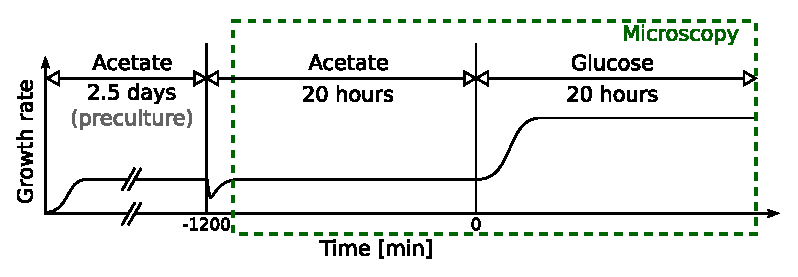
\includegraphics[scale=1]{./Fig/experiment_schema.eps}
\caption{The experiment. Caption to write.}
\label{fig:experiment_schema}
\end{figure}

\textbf{Note that several issues occurred during the experiment.
}\textit{
Out of focus during the night.
Cells die at the end of the experiment for an unknown reason, see discussion.
We use the exploitable part of the time scale, and get rid of out of focus images.
}

\textbf{The image analysis was done by focusing on the deepest cell in each well.
}\textit{Clicking at the pole on each image.
Defining a rectangle.
Figure about how we defined the rectangle.
The RFU, the length and the size must appear. Can be grouped with the last figure.
Correction background, closed shutter.
}

\begin{figure}[h!]
\centering
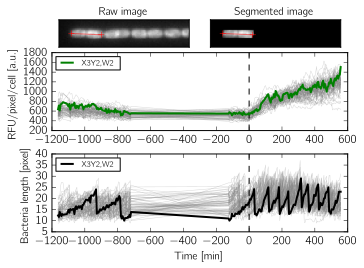
\includegraphics[scale=1]{./Fig/data_acquisition}
\caption{Result of the data acquisition. Caption to write.}
\label{fig:data_acquisition}
\end{figure}

\subsection{Data analysis using Kalman smoother}

\textbf{We have the bacteria size and RFU, but we want growth rate and gene expression machinery abundance.}
\textit{
They are several ways to obtain this information.
We will use Kalman smoothing.
}

\textit{
Kalman smoothing is a method that allow to do so and so, based on this principle, bayesian, blablabla.
}

\textit{
We state the problem as follows.
Gamma blablabla.
mu and alpha can be co-estimated, but we decided to first estimate mu than alpha because so and so.
}

\textit{
We generate synthetic data based on noise estimation (see supp info).
Can the kalman smoother estimate synthetic data for bang-bang?
Here figure with the synthetic data and the estimate.
}

\begin{figure}[h!]
\centering
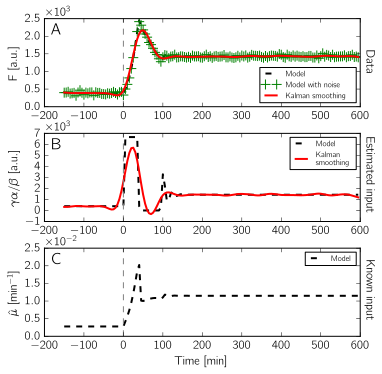
\includegraphics[scale=1]{./Fig/synthetic_upshift}
\caption{Synthetic data based on the model in Chapter 2. Caption to write.}
\label{fig:synthetic_upshift}
\end{figure}

\subsection{Estimation of the relevant parameters of the cell}

\subsubsection*{Growth rate estimation}

\textit{
Mu estimation is done by looking at the length, since bacteria can be modeled as cylinder.
We use such technique to identify discontinuities.
We use kalman smoother with such parameters, selected by trial and error.
There is a better way to do that (cross-validation) as is discussed in the discussion section.
We obtain these results.
Here a figure with the growth rate and estimation for one cell, and all the other cells in light background behind.
We comment the result.
As we can see there is a lot of variability, with some cells having a growth rate that goes to zero.
This probably reflects uncoherent behaviors, like cells dying before the end of the experiment.
Can we classify cells depending on their behavior?
}

\begin{figure}[h!]
\centering
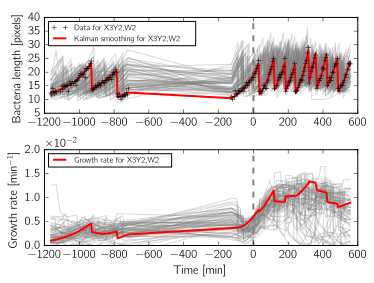
\includegraphics[scale=1]{./Fig/growth_rate_estimation}
\caption{Result of the growth rate estimation. Caption to write.}
\label{fig:growth_rate_estimation}
\end{figure}

\textit{
We identified 3 type of cells : normal, pausing, dying.
We list them (see supplementary information for details on individual cells).
We put a figure with an example for each type of cell, and the other in light gray in the background.
}

\begin{figure}[h!]
\centering
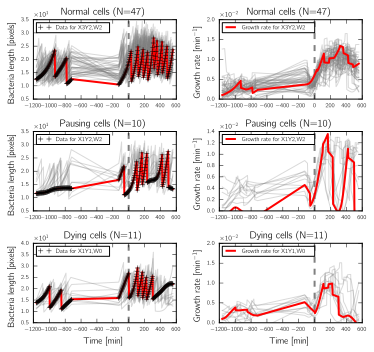
\includegraphics[scale=1]{./Fig/subcat_cells}
\caption{Subtypes of cells. Caption to write. Cutting the x axis might be a good idea because a third of the x-axis of each graph are "missing data".}
\label{fig:subcat_cells}
\end{figure}

\textit{
We focus on normal cells.
Here figure with the median, 5 percent and 95 percent curves (or 25 and 75) for the growth rate.
We comment the result for normal cells.
The growth rate increase after addition of glucose, that's neat.
}

\begin{figure}[h!]
\centering
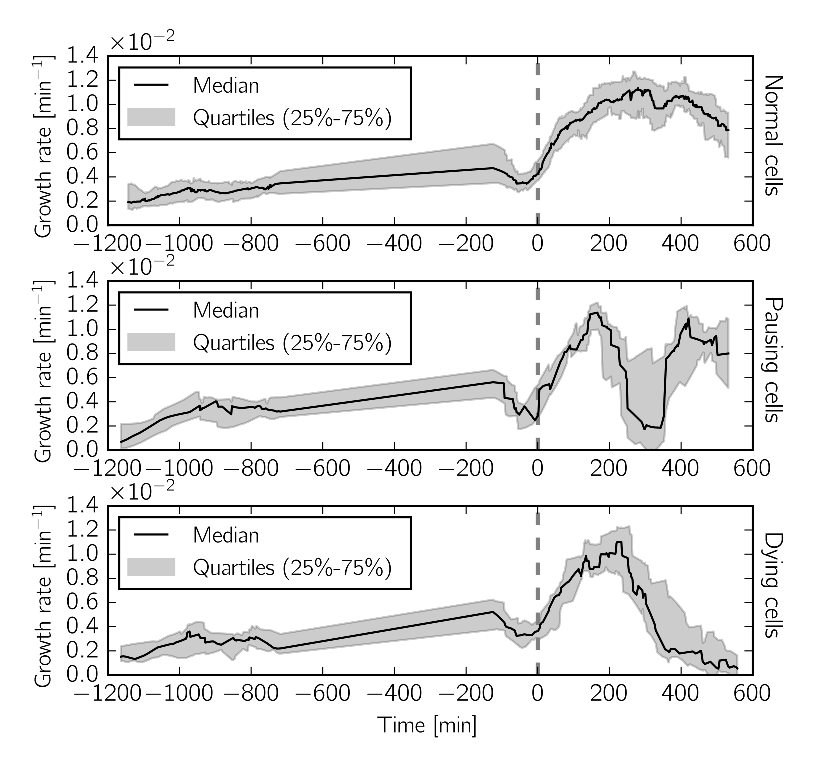
\includegraphics[scale=1]{./Fig/subcat_median}
\caption{Subtypes of cells, median. Caption to write.}
\label{fig:subcat_median}
\end{figure}

\subsubsection*{Estimation of gene activity}

\textit{
We use the mean RFU.
No need to identify discontinuities here since the signal is continuous.
We use kalman smoother on real cells with the same parameters.
Here figure with a typical cell.
We see strange fluctuations.
Not sure if they are real...
Comment comment.
}

\begin{figure}[h!]
\centering
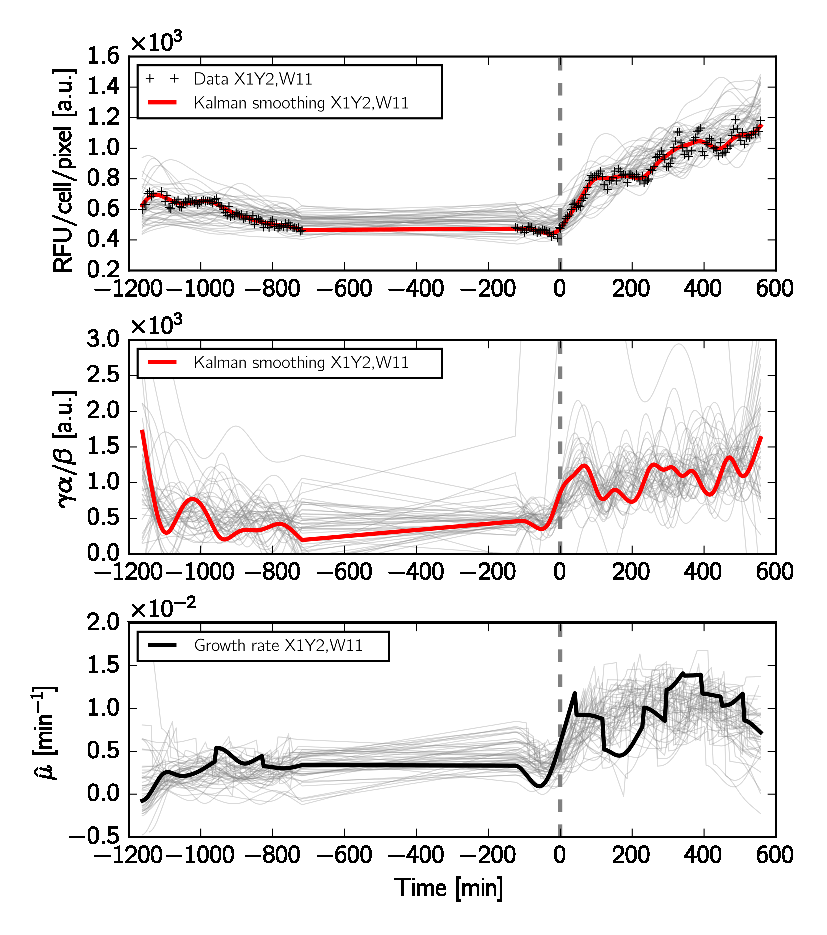
\includegraphics[scale=1]{./Fig/gene_activity}
\caption{Gene activity. Caption to write.}
\label{fig:gene_activity}
\end{figure}


\textit{
If we look at all the cells, we can plot the median and quartiles.
The first bang seems to be reproducible and synchronous.
That could represent what we expect, but be careful. See discussion.
}

\begin{figure}[h!]
\centering
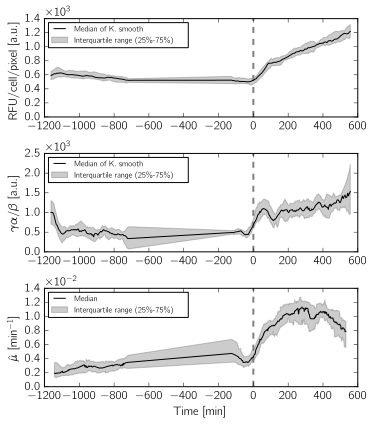
\includegraphics[scale=1]{./Fig/gene_activity_median}
\caption{Summary statistics for normal cells. Caption to write.}
\label{fig:gene_activity_median}
\end{figure}


\section{Discussion}

More research need to be done.

Could be interesting to use transitions for syn bio purposes.
Could be interesting to validate such results in different microorganisms, with different type of medium (fast env, slow env, etc)

\section{Material and Methods}

\subsection{Bacterial strain construction}

To achieve dynamical quantification of ribosome abundance, we designed and constructed a strain containing a translational fusion of \textit{gfpmut2}~\cite{zaslaver_comprehensive_2006} to the C-terminus of \textit{rpsB} (the gene coding the ribosome subunit S2).
This design was inspired by the work of Bakshi \textit{et al}, who used a similar construction to assess the quantitative spatial distribution of ribosomes in living \textit{E.~coli}~\cite{bakshi_superresolution_2012}.

The transcription factor \textit{tsf} is under the control of the same promoter than \textit{rpsB}, and is located after the C-terminus.
In order to ensure that \textit{tsf} expression was not affected by our translation fusion on \textit{rpsB}, we used a double-selection procedure to get rid of every resistance gene that the construction might introduce.
This is something that was not done in the original construction from Bakshi \textit{et al}~\cite{bakshi_superresolution_2012}

A DNA fragment containing a double selection cassette was amplified with two long primers annealing respectively to the region just after the STOP codon at the C-terminus of \textit{rpsB}, and to the beginning of \textit{gfpmut2}.
The double-selection cassette contained a resistance gene to Kanamycin (positive selection) and a gene coding for the CcdB toxin under the control of the P\textsubscript{BAD} promoter (negative selection in presence of Arabinose).
This cassette is referred below as \textit{kan-P\textsubscript{BAD}-ccdB}.

Another DNA fragment containing \textit{gfpmut2}~\cite{zaslaver_comprehensive_2006} without ATG was amplified with long primers annealing respectively to the C-terminus of rpsB (just before the STOP codon), and the end of the \textit{kan-P\textsubscript{BAD}-ccdB} cassette.
The first primer also contained a 18-bp (base pair) linker that was chosen according to the method section of~\cite{bakshi_superresolution_2012}.

Both fragments (the \textit{gfpmut2} reporter and the \textit{kan-P\textsubscript{BAD}-ccdB} cassette) were assembled using Gibson assembly~\cite{gibson_enzymatic_2009}.
Both PCR products were quantified using NanoDrop and mixed in equimolar proportions with a commercial Gibson Assembly Master mix.
A final product of 2683 bp was obtained:
\begin{itemize}
\item *(50 bp) the C-terminus of \textit{rpsB} without the STOP codon 
\item (18 bp) a linker (see Supporting Information)
\item (714 bp) the \textit{gfpmut2} sequence without the initial ATG
\item (1851 bp) the \textit{kan-P\textsubscript{BAD}-ccdB} cassette
\item *(50 bp) the region directly after \textit{rpsB} in \textit{E.~coli}
\end{itemize}
Regions labeled with * are expected to anneal with the \textit{E.~coli} chromosome.
The complete sequence of this fragment, as well as all the primers used are available in the Supporting Information of this chapter.

This fragment was electroporated in a BW25113 background strain containing the pSIM5 plasmid with chloramphenicol resistance (lambda-red recombinaison).
A kanamycin-resistant colony was selected and verified to exhibit green fluorescence in a Tecan microplate reader.
A new 100-bp fragment containing 50 bp of the end of \textit{gfpmut2} and 50 bp of the region just after \textit{rpsB} was electroporated into this strain (sequence available in Supporting Information) to get rid of the \textit{kan-P\textsubscript{BAD}-ccdB} cassette.
An arabinose-resistant colony was selected and verified to be kanamycin-sensitive and to still exhibit green fluorescence.
Finally, the strain was grown overnight at 42$^\circ$C to get rid of the pSIM5 plasmid and a chloramphenicol-sensitive colony was selected.
The region after \textit{rpsB} was verified by sequencing (full sequence available in Supporting Information).

In parallel, the same protocol was used to construct \textit{mCherry} and \textit{cfp} variants of the same strain.
However, only the \textit{gfpmut2} and \textit{mCherry} versions were successfully obtained for reasons that were not investigated.
The full sequence of the final \textit{rpsB-mCherry} strain is available in Supporting Information.

The \textit{rpsB-gfpmut2} and \textit{rpsB-mCherry} strains were characterized on different media using a Tecan microplate reader.
They were showed to exhibit a wild-type growth rate and sufficient fluorescence level to allow quantification.
However, the \textit{rpsB-mCherry} strain exhibited strange fluorescence dynamics, especially during growth transitions, which made it unsuitable for our study.
Our effort were then concentrated on the \textit{rpsB-gfp} strain.
Data as well as information on the matter are available in Supporting Information.

\subsection{Microfluidic device}

\textit{Irina gave me the relevant information about the microscope, the pump, the making of the microfluidic device, the auto-focus algorithm, etc.
Just need to rephrase everything.
We took 6 fields each containing 15 wells.}

\subsection{Cell segmentation}

\textit{We used OpenCV, scikit-image, and numpy in Python 3.5.
The raw 16-bit images given by the Olympus microscope were converted in 16-bit Tif format.
They were aligned using cross-correlation to correct for microscope drift.
Each well was cropped into an individual picture.
Only a single cell was segmented because we had trouble using available software with our experimental set-up (big pixels, reflection problem, fluorescence and phase contrast not aligned, not enough time...).
As a preliminary analysis, the segmentation was done manually by focusing on the poles of the deepest cell.
We used a rectangular mask around the cell with width of X pixels.
After applying the mask, we corrected the background by removing the mean of the noise (evaluated with a closed shutter, see supporting information).
We then computed the mean RFU in the mask (for ribosome concentration) and the lenght of the bacteria (for growth rate).
}

\subsection{Kalman smoothing}

\textit{We used Pandas and numpy to manipulate the data, and pykalman to perform the smoothing in Python 3.5.
Kalman smoother rely on this and that.
The following problem was considered :
[equations]
We used a double integral of the white noise because so and so.
}


\section{Supporting Information}

\begin{itemize}
\item Strain validation (signal-to-noise ratio, growth rate not hampered in microplate reader)
\item Primers used for gibson assembly
\item Difference between mCherry and GFP (mCherry not good because so and so, GFP was chosen)
\end{itemize}